\documentclass[a4paper]{article}

\usepackage[utf8]{inputenc}
\usepackage[T1]{fontenc}
\usepackage{textcomp}
\usepackage[english]{babel}
\usepackage{amsmath, amssymb}


% figure support
\usepackage{import}
\usepackage{xifthen}
\pdfminorversion=7
\usepackage{pdfpages}
\usepackage{transparent}
\usepackage{physics}
\graphicspath{ {./figures/} }
\setlength{\parindent}{0pt}
\usepackage{chngcntr}
\numberwithin{equation}{section}
\counterwithin{figure}{section}
\newcommand{\incfig}[1]{%
		\def\svgwidth{\columnwidth}
		\import{./figures/}{#1.pdf_tex}

}

\pdfsuppresswarningpagegroup=1

\begin{document}
\section{Introduction}



\section{Theory}


\section{Waveguides}
In order to understand cavities, we start off with the discussion on waveguides. An electromagnetic wave, when confined to the interior of a hollow pipe is called a waveguide. We shall closely follow the derivation from \cite{}.The generalized Maxwell equations in terms of E-field and H-field are given by:

\begin{align}
		\curl {\vb{{E}}} &= - \pdv{{B}}{t} \\
		\div{\vb{D}} &= \rho \\
		\curl {\vb{{H}}} &= \vec{j} + \pdv{{D}}{t} \\
		\div{\vb{{B}}} &= 0 
\end{align}

In vacuum, these equations become: 
\begin{align}
		\curl {\vb{{E}}} &= \mu_0 \cdot \pdv{{H}}{t} \\ 
		\div{\vb{{E}}} &= 0 \\
		\curl {\vb{{H}}} &= \epsilon_{0} \cdot \pdv{{E}}{t} \\
		\div{\vb{{H}}} &= 0
\end{align}

Upon solving these equations, we get plane wave solutions which looks like this: 
\begin{align*}
		\Delta \vec{E}\left(\vec{r}\right) + \frac{\omega}{c^2} \vec{E}\left(\vec{r}\right) = 0 \\
		\Delta \vec{B}\left(\vec{r}\right) + \frac{\omega}{c^2} \vec{B}\left(\vec{r}\right) = 0 
\end{align*}

Now, let us look at a waveguide which is aligned along the z-direction. Taking the ansatz $\vec{E} = \vec{E}(x,y).e^{i(\omega t -kz)}$ and the separation $\Delta = \Delta_{\perp} + \pdv[2]{}{z}$, for the longitudinal fields yields: 

\begin{align}
		\Delta_{\perp}E_{z} + k_{c}^2 E_{z} = 0 \\
		\Delta_{\perp}H_{z} + k_{c}^2 H_{z} = 0 
\end{align}
where 
\[
		k_{c}^2 = \frac{\omega^2 }{c^2 } - k^2   
\]
The quantity $k_{c} $ is called the critical wave number and is a characteristic property of the cavity, as we shall see. 
Solving these equations further, we see that it is sufficient to know the longitudinal fields, $E_{z} $ and $B_{z} $ because we can easily determine the transverse components from them. 
\begin{align} 
		ik_{c}^2 \vec{E}_{\perp} = k \vec{\nabla}_{\perp}E_{z} + \omega \mu _{0} \vec{\nabla}_{\perp}H_{z} \times \hat{e}_{z} \label{trans1} \\
		ik_{c}^2 \vec{H}_{\perp} = k \vec{\nabla}_{\perp}H_{z} - \omega \epsilon_{0} \vec{\nabla}_{\perp} E_{z} \times \hat{e}_{z} \label{trans2}     
\end{align}

Now, there are two waves to classify these waves: 
\begin{enumerate}
		\item $k_{c}^2 = 0  $ 
				\begin{enumerate}
						\item $\vec{\Delta_{\perp} }E_{z}  \ne 0$ and $\vec{\Delta}_{\perp}H_{z} \ne 0  $: HE or EH hybrid waves.
						\item $\vec{\Delta_{\perp} }E_{z}  = 0$ and $\vec{\Delta}_{\perp}H_{z} = 0  $: TEM waves.
				\end{enumerate}
		\item $k_{c}^2 \ne 0  $ 
		In this case we do not get any propagation if $\omega \leq c \cdot k_{c} $. These waves are called evanescent waves or the cut off condition. The possible propagation modes are: 
		\begin{enumerate}
				\item $E_{z}=0 $: TE (transversal electric) or H waves.
				\item $H_{z}=0 $: TM (transversal magnetic) or E waves.
		\end{enumerate}
		
\end{enumerate}

Corresponding to this critical wave, we have a critical frequency, which is $\omega_{c}=k_{c}.c $, below which there is no propagation. 
One interesting thing to note here is that for a hollow waveguide, only TE or TM modes are possible, TEM is not, because no wave would exist in this case \cite{}. But for a coaxial cable, which consists of straight wire surrounded by a conduction sheath, we can get TEM modes.

\subsection{Cylindrical waveguides}
We now consider a cylindrical waveguide with an inner radius a. This imposes the following boundary conditions to the walls of the waveguide:
\begin{itemize}
		\item $E_{\phi} = 0$, $E_{z} = 0 $ \text{for} $r = a$ 
		\item $H_{r} = 0 $ \text{for} $r = a$ 
\end{itemize}

The field distribution solution for a cylindrical waveguide can be separated into angular and radial parts, whose solutions are then given by the Bessel/Neumann functions. These can be then substituted in the eq.(\ref{trans1})-(\ref{trans2}) and upon imposing the constraints from the boundary condition gives us the corresponding TE- and TM-modes.

\subsection{Cylindrical waveguides resonator}
The time has now come, to talk about cavities itself. If we now insert two conducting plates perpendicular to the z-axis, the incoming wave is reflected completely, giving us standing waves. Because of this, the z-dependence changes like: 

\[
		a \cdot e^{ikz} \implies A \cdot \sin\left(kz + \phi_{0}\right)    
\]
The following condition is imposed so that the longitudinal boundary conditions are fulfilled: $k = p\cdot \pi /l $. The longitudinal field looks like: 
\begin{align*}
		\mathbf{TE_{mnp}-Modes}: H_{z} = H_{mn}\cdot J_{m} \left(k_{c}r \right) \cos\left(m \phi \right) \cdot \sin\left(p \pi / l \cdot z \right) \cdot e^{\omega_{mnp}t} \text{ where } k_{c}a=j_{mn}^{'}  \\
		\mathbf{TM_{mnp}-Modes}: E_{z} = E_{mn}\cdot J_{m}^{'}  \left(k_{c}r \right) \cos\left(m \phi \right) \cdot \cos\left(p \pi / l \cdot z \right) \cdot e^{\omega_{mnp}t} \text{ where } k_{c}a=j_{mn} 
\end{align*}
For resonant frequency, we have:

\[
		\omega_{mnp} = c \cdot \sqrt{\left(j_{mn}/a\right)^2 + \left(p \pi / l\right)^2} 
\]

Here, $J_{m}$ is the $m$-th Bessel function, $J_{m}^{'} $ is its derivative. And $j_{mn}$ and $j_{mn}^{'}$ are the $n$-th zeropoints of the $m$-th Bessel function and its derivative.

The resonant modes can be written in the linear form as:

\begin{equation}
		\left(d \nu \right)^2 = \left(\frac{cj_{mn}^{(')}}{\pi}\right)^2 + \left(\frac{c}{2}\right)^2 p^2 \left(\frac{d}{l}\right)^2
\end{equation}

here $d$ is the diameter of the cavity.
When we plot different modes on a graph, we get a mode map (Fig.\ref{fig:mode}). The mode map allows one to read off the resonant frequencies for different diameters and length of the cavity. 

\begin{figure}[htpb]
    \centering
    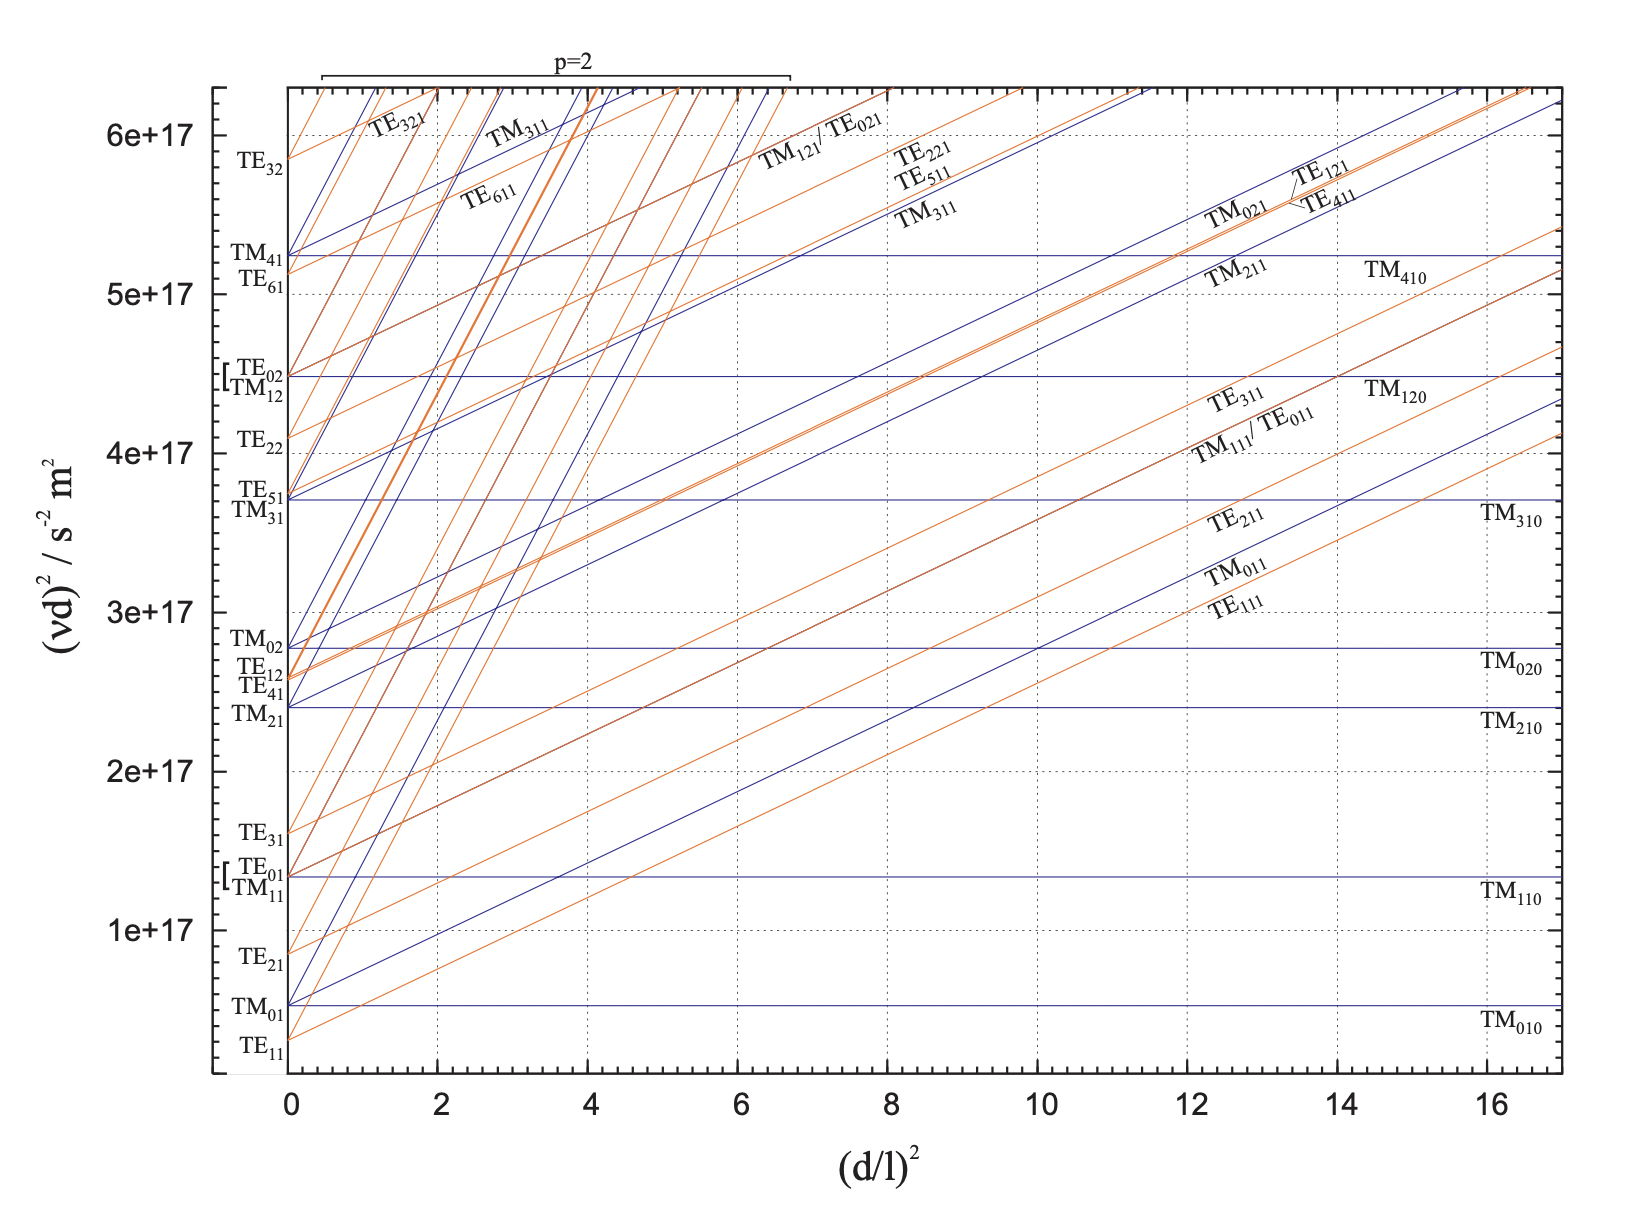
\includegraphics[width=0.8\textwidth]{mode_map}
    \caption{Mode map for $p \leq 2$ \ref{} }
    \label{fig:mode}
\end{figure}

Since the derivative of the zeroth order Bessel function and the first order Bessel function, $j^{'}_{0n}$ and $j_{1n}$, are equal, the corresponding TE- and TM-modes have the same resonant frequencies. That is, $TE_{0np}$-modes and $TM_{1np}$-modes have the same resonant frequency. 

\section{Oscillating circuit}
A cavity has a lot of characteristic quantities, which can be described by an equivalent circuit (Fig.\ref{fig:circuit}). 
\begin{figure}[htpb]
    \centering
    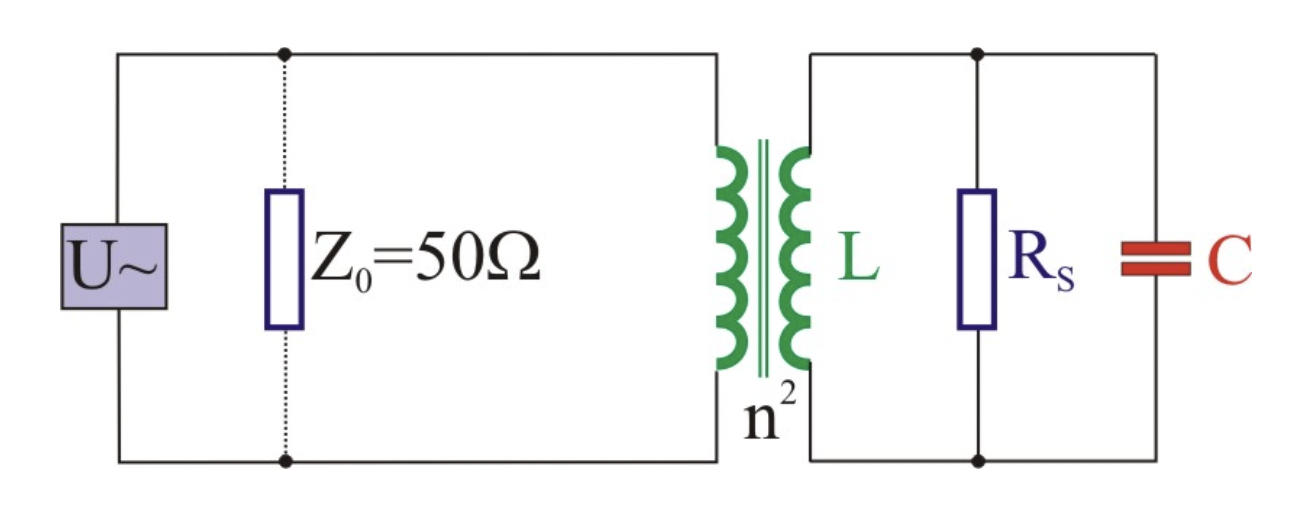
\includegraphics[width=0.8\textwidth]{circuit}
    \caption{Equivalent circuit of a cavity with loop coupling}
    \label{fig:circuit}
\end{figure}	

Coupling is a process through which electromagnetic waves can be coupled to a waveguide, or in this case, to a cavity. There are several ways to couple and in this experiment, we use loop coupling, which enables coupling to the magnetic field inside the cavity. In the figure \ref{fig:circuit}, the LCR-circuit represents the cavity. The step-down transformer represents the loop coupling, $Z_{0}$ is the characteristic impedance and $R_{s}$ is the Shunt impedance. 

The characteristic quantities associated with the cavity are:
\begin{itemize}
		\item Quality factor 
		\item Coupling coefficient 
		\item Reflection coefficient 
		\item Shunt impedance
\end{itemize}

Let us look at these quantities in a bit more detail. 

\subsection{Quality factor}
Quality factor is a dimensionless quantity which describes how underdamped an oscillator or resonator is. It is defined as: 
\begin{equation}
		Q_{0} = \frac{2 \cdot \pi \text{stored energy} }{\text{losses per period}} = \frac{2 \pi \cdot W }{T\cdot P} =  \frac{\omega_{0}\cdot W}{P}
\end{equation}
where $\omega_{0}$ is the angular resonant frequency. 
Looking at the case of driven oscillations, the unloaded quality factor can be determined from the Full Width Half Maximum (FWHM), $\Delta \omega_{H}$

\begin{equation}
		Q_{0} = \frac{\omega_{0}}{\Delta \omega_{H}}
\end{equation}

\subsection{Coupling coefficient}
The coupling coefficient is defined as:
\begin{equation}
		\kappa = \frac{Z_{a}}{Z_{0}} = \frac{R_{s}}{n^2Z_{0}} = \frac{Q_{0}}{Q_{ext}}	
\end{equation}
where $n$ is the transformer turn ratio, $Q_{0}$ is the unloaded quality factor and $Q_{ext}$ is the external quality factor.  
If we know the coupling coefficient, the unloaded quality factor can be calculated using: 
\begin{equation}
		Q_{0} = \left(1 + \kappa\right)\cdot Q
\end{equation}

We also get 3 cases for the coupling coefficient, which are: 

\begin{itemize}
		\item $\kappa < 1$: undercritical coupling, $Q>Q_{0}/2$
		\item $\kappa = 1$: critical coupling, $Q = Q_{0}/2$ (no reflection)
		\item $\kappa > 1$: overcritical coupling, $Q<Q_{0}/2$ 
\end{itemize}

\subsection{Reflection coefficient}
In the conductor, we have an incoming wave ($\hat{U}_{+}, \hat{I}_{+}$) and reflected wave ($\hat{U}_{-}, \hat{I}_{-}$). Hence we define the complex reflection coefficient as:

\begin{equation}
		\rho = \frac{\hat{U}_{-}}{\hat{U}_{+}}
\end{equation}

The coupling coefficient and the reflection coefficient are related at resonance by: 
\begin{equation}
		\kappa = \left|\frac{1 + \rho}{1 - \rho} \right| 
\end{equation}
We shall discuss more about this in the next section.

\subsection{Shunt impedance}
Shunt impedance tells us how much energy is gained by a charged particle when it crosses the cavity. It is defined by: 

\begin{equation}
		R_{s} = \frac{U^2}{2 P_{V}} = \frac{1}{P_{V}} \left|\int\limits_{L/2}^{-L/2} E_{0}\left(s \right) \cdot e^{i \omega_{0}s/c}\cdot ds \right|^2 
\end{equation}


\end{document}
